\documentclass[../main.tex]{subfile}

\begin{document}

\section{Численное решение алгебраических уравнений}

Предположим, что нам нужно решить в действительных числах уравнение
$y(x)=0$. Если это просто абстрактное уравнение, то нет единого
алгоритма, как его решить. Первое, что можно сделать -- это локализовать
корни, но это можно сделать лишь по виду функции.

\subsection{Метод бисекции}

Простейший метод отыскания нуля функции -- это метод бисекции, или метод
деления отрезка пополам. Для него нужна лишь совсем небольшая математическая
база.

\begin{algorithm}[метод бисекции]
	Необходимо найти ноль функции $f(x)$ на отрезке $[a,b]$ таком, что:
	\begin{enumerate}[noitemsep, nolistsep]
		\item $f(x)\in C([a,b])$;
		\item $f(a)f(b)<0$, то есть на концах отрезка функция
			принимает значения, противоположные по знаку.
	\end{enumerate}\leavevmode\newline

	Организуем систему вложенных отрезков $[a_n, b_n]$ так, что\\
	$[a_1, b_1]=[a,b]$, а следующие отрезки сформированы следующим образом:
	если $c_k=\frac{a_k+b_k}{2}$, то:
	\begin{itemize}[noitemsep, nolistsep]
		\item Если $f(c_k)=0$, то мы нашли корень, можно не продолжать;
		\item В противном случае, мы берём тот конец отрезка, функция от
			которой не совпала по знаку с $f(c_k)$, и формируем из него
			и точки $c_k$ отрезок $[a_{k+1},b_{k+1}]$.
	\end{itemize}

	Условие выхода: $|f(c_n)|<\varepsilon$, где $\varepsilon>0$ -- некоторая
	погрешность.

	Если данный алгоритм усилить монотонным возрастанием или убыванием на $[a,b]$,
	то ноль на нём будет единственный.
\end{algorithm}

Корректность данного алгоритма напрямую следует из теоремы Больцано-Коши, которая
и доказывается методом бисекции в сочетании с теоремой о двух милиционерах.

\begin{example}
	Пусть нужно решить уравнение
	\[f(x)=x^3-6x^2+8x+2=0.\]

	Функция непрерывна на всей вещественной оси. Значит, с локализацией
	корней проблем быть не должно.
	\newline

	\begin{tabular}{ |c|c|c|c|c| }
		\hline
		$x$		& 0	& 1	& 2	& 3 \\
		\hline
		Знак $f(x)$ 	& $+$	& $+$	& $+$	& $-$ \\
		\hline
	\end{tabular}
	\newline

	%TODO найти команду, которую находит значения функции в точке (параметры: функция и точка)
	Тогда $\exists c\in[2,3]: f(c)=0$. Найдём его методом бисекции:
	\begin{itemize}[noitemsep, nolistsep]
		\item $f(2.5)=0.125>0$, ищем на $[2.5,3]$;
		\item $f(2.75)\approx -0.5781<0$, ищем на $[2.5,2.75]$;
		\item $f(2.625)\approx -0.2259<0$, ищем на $[2.5,2.625]$ и т. д.
	\end{itemize}

	На графике это выглядит вот так:
	\newline

	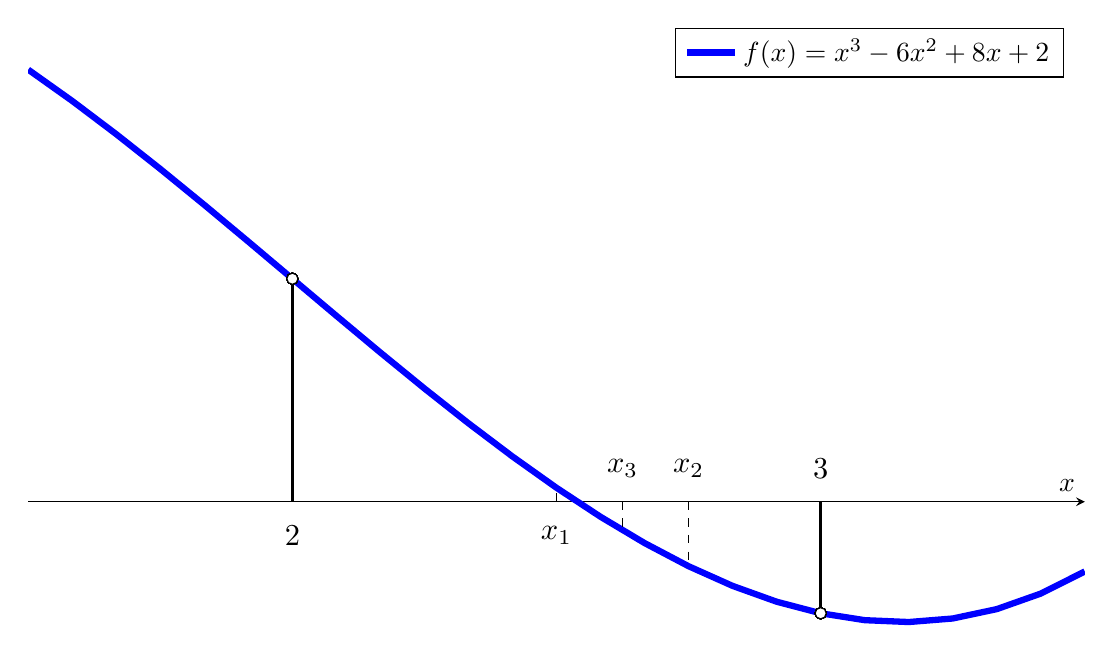
\begin{tikzpicture} [
		declare function={
			f(\x)= \x^3 - 6*\x^2+ 8*\x + 2;
		},
	]
		\begin{axis} [
			height=10cm,
			width=15cm,
			xlabel = {$x$},
			ylabel = {$f(x)$},
			axis x line = middle,
			hide y axis,
			domain = 1.5:3.5,
			ticks = none ]

			\addplot[color=blue, line width=.08cm]{f(x)};

			\addplot[mark=*,only marks, fill=white] (2,2)
				node[above, pos=1]{};
			\addplot[mark=*,only marks, fill=white] (3,-1)
				node[above, pos=1]{};

			\draw[very thick,black] (2,0) -- (2,2);
			\draw[very thick,black] (3,0) -- (3,-1);
			\draw[dashed,black] (2.5,0) -- (2.5,0.125);
			\draw[dashed,black] (2.75,0) -- (2.75,-0.5781);
			\draw[dashed,black] (2.625,0) -- (2.625,-0.2259);

			\node[scale=1.1] at (2,-.3) {$2$};
			\node[scale=1.1] at (3,.3) {$3$};
			\node[scale=1.1] at (2.5,-.3) {$x_1$};
			\node[scale=1.1] at (2.75,.3) {$x_2$};
			\node[scale=1.1] at (2.625,.3) {$x_3$};

			\addlegendentry{$f(x)=x^3-6x^2+8x+2$}
		\end{axis}
	\end{tikzpicture}
\end{example}


\subsection{Итерационные методы решения алгебраических уравнений}

Метод бисекции гарантированно даёт нам результат. Но нам бы хотелось иметь
более быструю сходимость. В этом нам могут помочь итерационные методы.

\begin{define}
	\textbf{Итерацией} называется многократное применение одной и той же
	функции $f$ к числу. Пусть задано начальное число $x_0$, тогда:
	\begin{itemize}[noitemsep, nolistsep]
		\item $x_1=f(x_0)$,
		\item $x_2=f(x_1)=f(f(x_0))$,\\
		...
		\item $x_n=f(x_{n-1})=\underset{n}{\underbrace{f(f(...f}}(x_0)...))$.
	\end{itemize}

	\textbf{Последовательность} $\{x_n\}$, образованная таким образом,
	называется \textbf{итерационной} с базой $x_0$ и функцией итерации $f(x)$.
\end{define}

\begin{algorithm}[метод простой итерации]
	Пусть нужно решить уравнение $y(x)=0$. Сделаем подстановку
	$g(x)=x+\tau y(x)$, где $\tau$ -- некоторая положительная константа.
	Таким образом, теперь нужно решить уравнение $g(x)=x$, то есть вместо
	нулей функции мы ищем неподвижные точки.

	Пусть $x_0$ -- некоторое начальное приближение. Построим итерационную
	последовательность с базой $x_0$ и функцией итерации $g(x)$. Если
	параметр $\tau$ подобран правильно, итерационная последовательность
	сойдётся к неподвижной точке. При заданной погрешности $\varepsilon$
	завершаем итерацию при $|g(x_n)-x_n|<\varepsilon$.
\end{algorithm}

Как нужно подобрать $\tau$, чтобы последовательность сошлась? Однозначного ответа
нет. Однако тут частично выручает та теория, которую мы узнали на ДГМА. Дело
идёт о так называемых сжимающих операторах.

Для начала не помешает освежить в своей памяти некоторые определения.

\begin{define}
	\textbf{Метрическим пространством} называется пространство $M$, в
	котором определена операция метрики $\rho: M^2 \rightarrow \mathbb R $
	такая, что $\forall x, y, z \in M$ верно
	\begin{enumerate}[noitemsep, nolistsep]
		\item $\rho(x,y)\ge 0$, причём $\rho(x,y) = 0 \Leftrightarrow x=y$;
		\item $\rho(x,y)=\rho(y,x)$;
		\item $\rho(x,y)\le \rho(x,z) + \rho(z,y)$.
	\end{enumerate}

	Если дополнительно верно, что каждая фундаментальная последовательность
	$M$ сходится к элементу, принадлежащему ему, то $M$ --
	\textbf{полное метрическое пространство}.
\end{define}

\begin{define}
	\textbf{Сжимающим оператором} на метрическом пространстве $M$ с метрикой
	$\rho$ называется оператор $f: M \rightarrow M$ такой, что\\
	$\exists q \in(0;1):\forall x,y \in M\;\; \rho(f(x),f(y)) \le q \rho(x,y)$.

	Число $q$ назовём \textbf{коэффициентом сжатия}.
\end{define}

\begin{theorem}[о сжимающем операторе]
	Пусть $(M,\rho)$ -- полное метрическое пространство, $f$ -- сжимающий
	оператор на $M$ с коэффициентом сжатия $q$. Тогда:
	\begin{enumerate}[noitemsep, nolistsep]
		\item $\exists!\;\widetilde{x}\in M: f(\widetilde{x})=\widetilde{x}$;
		\item Любая последовательность $\{x_n\}$ такая, что $x_0 \in M$ --
			произвольный, $x_{k+1}=f(x_k)$, сходится к $\widetilde{x}$;
		\item Для всякой такой последовательности верно\\
			$\rho(x_n, \widetilde{x}) \le q ^ n \rho(x_0, \widetilde{x})$.
	\end{enumerate}
\end{theorem}

Данная теорема была доказана в курсе "Дополнительные главы математического анализа"{}.
В литературе эта теорема также известна как "Теорема Банаха о неподвижной точке"{}.

Всё это нужно было для того, чтобы доказать красивую, но практически бесполезную
теорему.

\begin{theorem}[о сходимости итерационного процесса]
	Пусть нам необходимо найти неподвижную точку функции $g(x)$. Зададим
	в качестве полного метрического пространства отрезок $G=\{x: |x-a| \le r\}$,
	где $a$ и $r$ -- параметры отрезка. Для того чтобы итерационный процесс
	$x_{k+1}=g(x_k)$ сошёлся, достаточно, чтобы:
	\begin{enumerate}[noitemsep, nolistsep]
		\item $\forall x,y\in G\;|g(x)-g(y)|\le q|x-y|$, где $q\in(0,1)$ --
			некоторая константа, то есть верно условие Липшица;
		\item $|g(a)-a|\le(1-q)r$.
	\end{enumerate}
\end{theorem}

\beginproof

	Нам всего лишь нужно доказать, что $g(x)$ замкнута на $G$.
	\begin{multline*}
		\forall x\in G:|g(x)-a|=|g(x)-g(a)+g(a)-a|\le \\
		\le|g(x)-g(a)|+|g(a)-a|.
	\end{multline*}

	Применив условия 1 и 2 к первому и второму модулю соответственно, получаем
	\begin{align*}
		|g(x)-g(a)|+|g(a)-a|\le q|x-a|+(1-q)r\le qr+r-qr=r.
	\end{align*}

	Следовательно, $\forall x\in G: |g(x)-a|\le r\Rightarrow\forall x\in G\;\;g(x)\in G$,
	что и даёт нам замкнутость $g(x)$ на этом отрезке. Условие 1 и замкнутость
	даёт нам право считать $g(x)$ сжимающим отображением, поэтому тут применима
	теорема Банаха о неподвижной точке -- итерационный процесс сходится.\qed


\begin{example}[графическая интерпретация метода простой итерации]
	Нужно решить уравнение \(e^x=x+2.\) Как и в предыдущем примере, с
	непрерывностью у данной функции проблем нет.

	Отобразим функции $g(x)=e^x$ и $h(x)=x+2$ на графике:
	\newline

	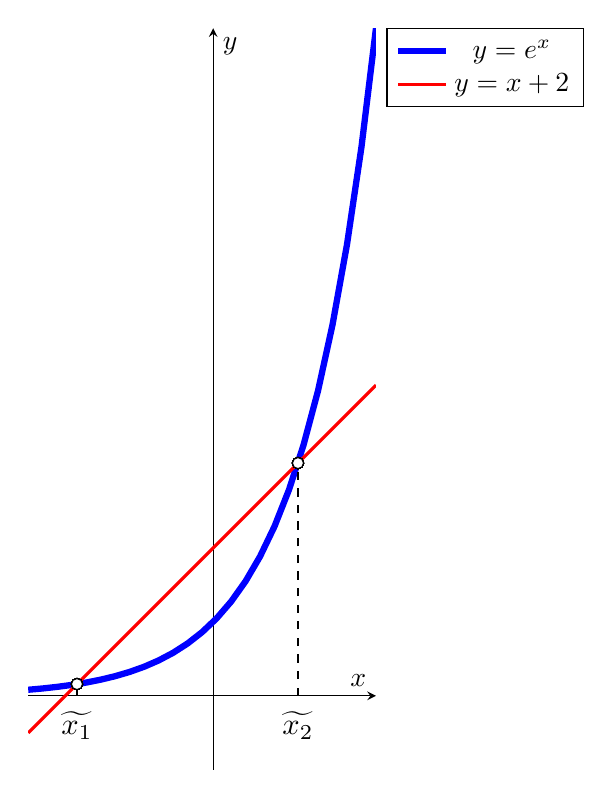
\begin{tikzpicture}
		\begin{axis} [
			unit vector ratio*=1 1,
			%width=11cm,
			height=11cm,
			xlabel = {$x$},
			ylabel = {$y$},
			axis x line = middle,
			axis y line = middle,
			domain = -2.5:2.2,
			ymin = -1,
			ticks = none,
			legend pos = outer north east]

			\addplot[color=blue, line width=.08cm]{e^x};
			\addplot[color=red, line width=.04cm]{x+2};

			\addplot[mark=*,only marks, fill=white] (1.146,3.146)
				node[above, pos=1]{};
			\addplot[mark=*,only marks, fill=white] (-1.841,0.159)
				node[above, pos=1]{};

			\draw[dashed,black] (1.146,0) -- (1.146,3.146);
			\draw[dashed,black] (-1.841,0) -- (-1.841,0.159);

			\node[scale=1.1] at (1.146,-.4) {$\widetilde{x_2}$};
			\node[scale=1.1] at (-1.841,-.4) {$\widetilde{x_1}$};

			\addlegendentry{$y=e^x$};
			\addlegendentry{$y=x+2$};
		\end{axis}
	\end{tikzpicture}
	\newline

	Видно, что у уравнения имеются 2 решения. Обозначим их как $\widetilde{x_1}$
	и $\widetilde{x_2}$. Запишем уравнение так, будто мы ищем нули функции:
	$f(x) = e^x-x-2$. Теперь локализуем корни:
	\newline

	\begin{tabular}{ |c|c|c|c|c|c| }
		\hline
		$x$		& -2	& -1	& 0	& 1	& 2 \\
		\hline
		Знак $f(x)$ 	& $+$	& $-$	& $-$	& $-$ 	& $+$\\
		\hline
	\end{tabular}
	\newline

	$\widetilde{x_1}\in[-2,-1],\;\widetilde{x_2}\in[1,2]$.

	\newpage
	Теперь запишем уравнение через поиск неподвижной точки, то есть как
	$u(x)=e^x-2$.

	Найдём сначала $\widetilde{x_1}$. За начальную точку возьмём $x_1=-1.5$ --
	середину отрезка. Поехали:
	\begin{itemize}[noitemsep, nolistsep]
		\item $x_1=u(-1.5000)\approx -1.7769$, $|u(x_0)-x_0|\approx 0.2769$;
		\item $x_2=u(-1.7769)\approx -1.8308$, $|u(x_1)-x_1|\approx 0.0539$;
		\item $x_3=u(-1.8308)\approx -1.8397$, $|u(x_2)-x_2|\approx 0.0089$ и т. д.
	\end{itemize}

	Итерационная последовательность очень быстро сходится к $\widetilde{x_1}$. Не менее
	интересно будет посмотреть на это на графике:
	\newline

	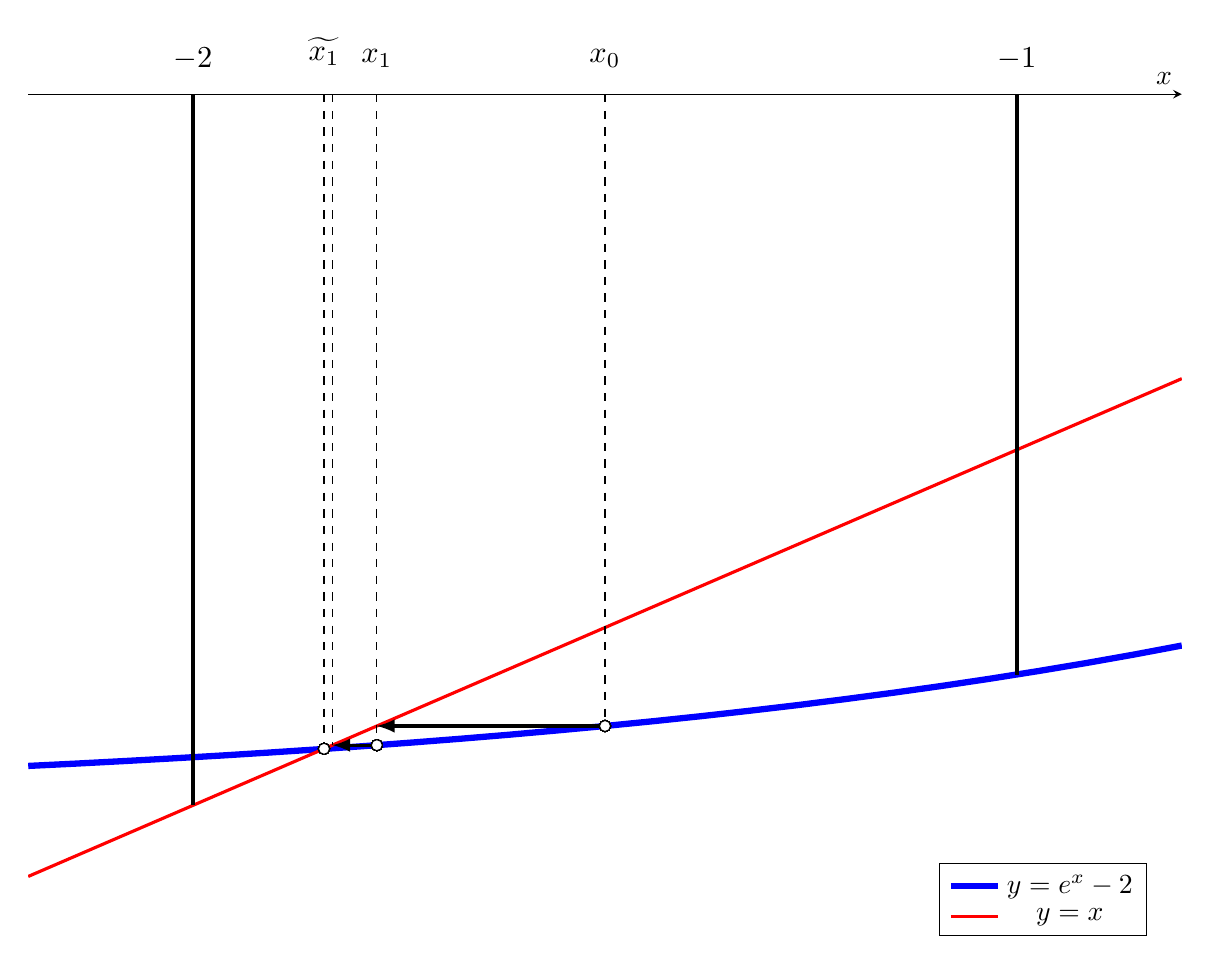
\begin{tikzpicture}
		\begin{axis} [
			height=14cm,
			xlabel = {$x$},
			ylabel = {$y$},
			axis x line = middle,
			hide y axis,
			ymax = 0.3,
			domain = -2.2:-0.8,
			ticks = none,
			legend pos = south east ]

			\addplot[color=blue, line width=.08cm]{e^x - 2};
			\addplot[color=red, line width=.04cm]{x};

			\addplot[mark=*,only marks, fill=white] (-1.841,-1.841)
				node[above, pos=1]{};
			\addplot[mark=*,only marks, fill=white] (-1.5,-1.7769)
				node[above, pos=1]{};
			\addplot[mark=*,only marks, fill=white] (-1.7769,-1.8308)
				node[above, pos=1]{};

			\draw[very thick,black] (-2,0) -- (-2,-2);
			\draw[very thick,black] (-1,0) -- (-1,-1.6321);
			\draw[dashed,black] (-1.841,0) -- (-1.841,-1.841);
			\draw[dashed,black] (-1.5,0) -- (-1.5,-1.7769);
			\draw[dashed,black] (-1.7769,0) -- (-1.7769,-1.8308);
			\draw[dashed,black] (-1.8308,0) -- (-1.8308,-1.8308);

			\draw[-latex, black, very thick] (-1.5, -1.7769) -- (-1.7769, -1.7769);
			\draw[-latex, black, very thick] (-1.7769, -1.8308) -- (-1.8308, -1.8308);

			\node[scale=1.1] at (-2,0.1) {$-2$};
			\node[scale=1.1] at (-1,0.1) {$-1$};
			\node[scale=1.1] at (-1.841,0.12) {$\widetilde{x_1}$};
			\node[scale=1.1] at (-1.5,0.1) {$x_0$};
			\node[scale=1.1] at (-1.7769,0.1) {$x_1$};

			\addlegendentry{$y=e^x-2$};
			\addlegendentry{$y=x$};
		\end{axis}
	\end{tikzpicture}
	\newpage

	Теперь попробуем найти $x_2$, который где-то на отрезке $[1,2]$. Как и
	в предыдущем случае, за $x_0$ возьмём середину отрезка, то есть 1.5:
	\begin{itemize}[noitemsep, nolistsep]
		\item $x_1=u(1.5000)\approx 2.4817$, $|u(x_0)-x_0|\approx 0.9817$;
		\item $x_2=u(2.4817)\approx 9.9616$, $|u(x_1)-x_1|\approx 7.4799$;
	\item $x_3=u(9.9616)\approx 21194.68329$ и т. д.
	\end{itemize}

	Вот тут нам не повезло: итерационная последовательность разошлась.
	На это тоже можно посмотреть на графике:
	\newline

	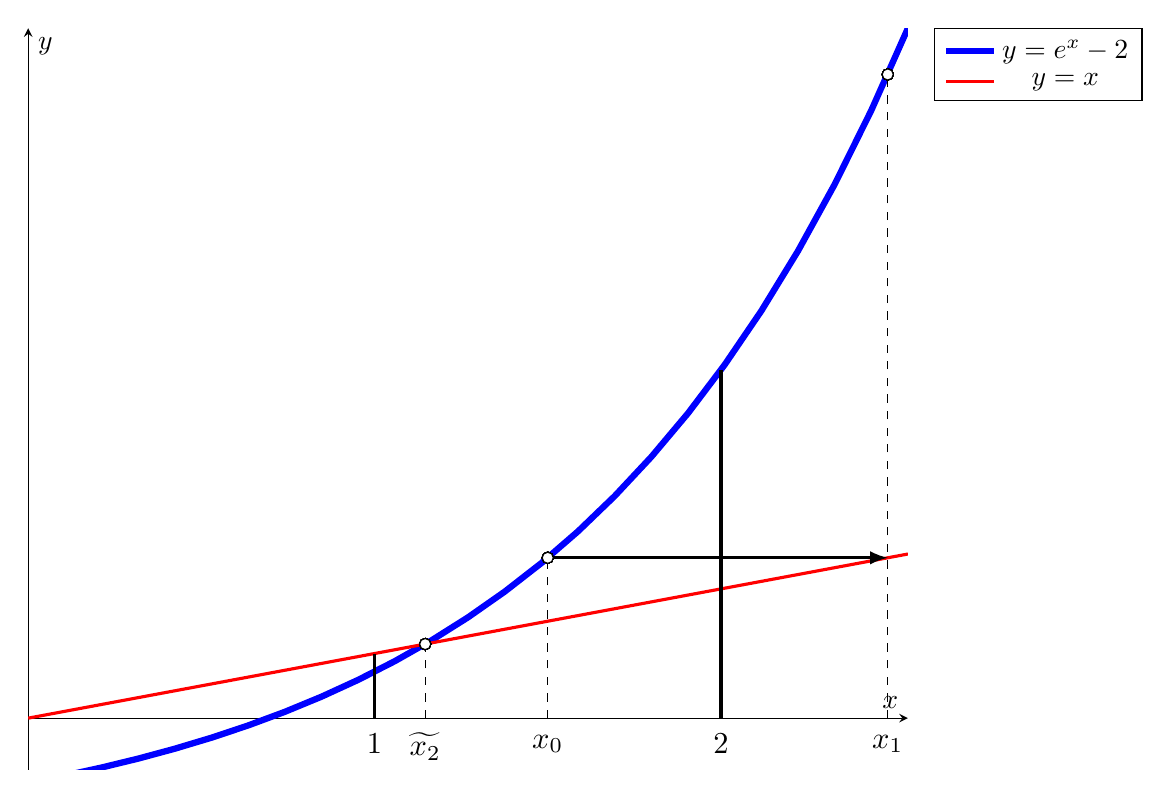
\begin{tikzpicture}
		\begin{axis} [
			height=11cm,
			xlabel = {$x$},
			ylabel = {$y$},
			axis x line = middle,
			axis y line = middle,
			ymin = -0.8,
			domain = 0:2.54,
			ticks = none,
			legend pos = outer north east
		]
			\addplot[color=blue, line width=.08cm]{e^x - 2};
			\addplot[color=red, line width=.04cm]{x};

			\addplot[mark=*,only marks, fill=white] (1.1462,1.1462)
				node[above, pos=1]{};
			\addplot[mark=*,only marks, fill=white] (1.5,2.4817)
				node[above, pos=1]{};
			\addplot[mark=*,only marks, fill=white] (2.4817,9.9616)
				node[above, pos=1]{};

			\draw[very thick,black] (1,0) -- (1,1);
			\draw[very thick,black] (2,0) -- (2,5.3891);
			\draw[dashed,black] (1.1462,0) -- (1.1462,1.1462);
			\draw[dashed,black] (1.5,0) -- (1.5,2.4817);
			\draw[dashed,black] (2.4817,0) -- (2.4817,9.9616);

			\draw[-latex, black, very thick] (1.5, 2.4817) -- (2.4817, 2.4817);

			\node[scale=1.1] at (1,-0.4) {$1$};
			\node[scale=1.1] at (2,-0.4) {$2$};
			\node[scale=1.1] at (1.14620,-0.44) {$\widetilde{x_2}$};
			\node[scale=1.1] at (1.5,-0.4) {$x_0$};
			\node[scale=1.1] at (2.4817,-0.4) {$x_1$};

			\addlegendentry{$y=e^x-2$};
			\addlegendentry{$y=x$};
		\end{axis}
	\end{tikzpicture}

	Во втором случае расхождение последовательности произошло из-за того, что
	производная $\forall x\ge 1: |u'(x)|>1$.
\end{example}

Однако невыполнение условий теоремы ещё не означает, что итерационная
последовательность не сойдётся к неподвижной точке.

\begin{example}
	Необходимо найти неподвижные точки функции \[f(x)=-e^{2x}+4.5e^x-3.\]

	Предположим, мы уже локализовали одну неподвижную точку на отрезке $[-1,0]$.
	Взяв $x_0$ равным -0.5, начнём строить итерационную последовательность:

	\begin{enumerate}[noitemsep, nolistsep]
		\item $x_1\approx -0.6385, |f(x_0)-x_0|\approx 0.1385$,
		\item $x_2\approx -0.9025, |f(x_1)-x_1|\approx 0.2640$,
		\item $x_3\approx -1.3395, |f(x_2)-x_2|\approx 0.4370$,
		\item $x_4\approx -1.8897, |f(x_3)-x_3|\approx 0.5502$,
		\item $x_5\approx -2.3428, |f(x_4)-x_4|\approx 0.4531$,
		\item $x_6\approx -2.5770, |f(x_5)-x_5|\approx 0.2342$,
		\item $x_7\approx -2.6638, |f(x_6)-x_6|\approx 0.0868$,
		\item $x_8\approx -2.6913, |f(x_7)-x_7|\approx 0.0275$,
		\item $x_9\approx -2.6995, |f(x_8)-x_8|\approx 0.0082$, и т. д.
	\end{enumerate}\leavevmode

	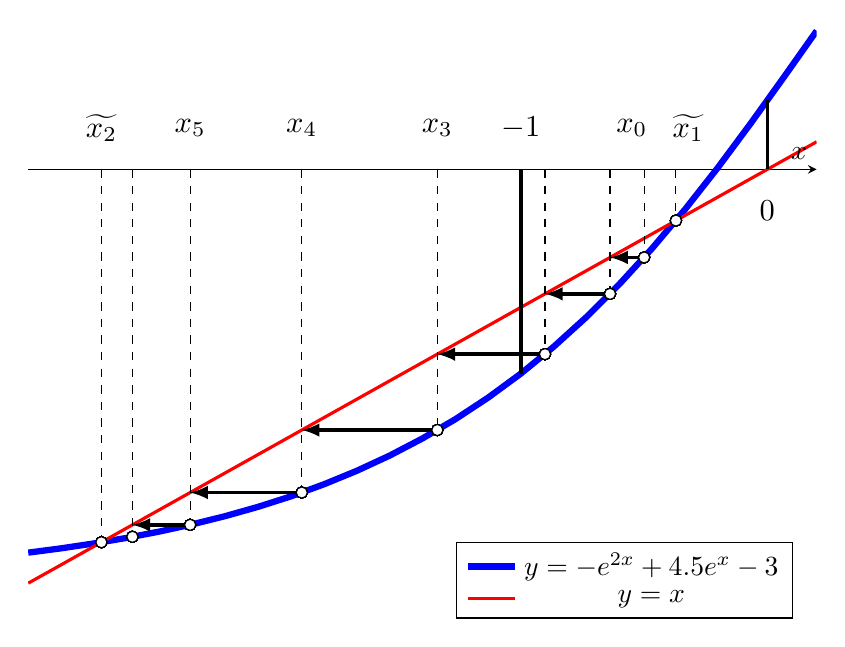
\begin{tikzpicture}
		\begin{axis} [
			height=10cm,
			xlabel = {$x$},
			ylabel = {$y$},
			axis x line = middle,
			hide y axis,
			domain = -3:0.2,
			ticks = none,
			legend pos = south east]

			\addplot[color=blue, line width=.08cm]{-e^(2*x) + 4.5*e^x - 3};
			\addplot[color=red, line width=.04cm]{x};


			\addplot[mark=*,only marks, fill=white] (-0.371, -0.371)
				node[above, pos=1]{};
			\addplot[mark=*,only marks, fill=white] (-2.703, -2.703)
				node[above, pos=1]{};
			\addplot[mark=*,only marks, fill=white] (-0.5000,-0.6385)
				node[above, pos=1]{};
			\addplot[mark=*,only marks, fill=white] (-0.6385,-0.9025)
				node[above, pos=1]{};
			\addplot[mark=*,only marks, fill=white] (-0.9025,-1.3395)
				node[above, pos=1]{};
			\addplot[mark=*,only marks, fill=white] (-1.3395,-1.8897)
				node[above, pos=1]{};
			\addplot[mark=*,only marks, fill=white] (-1.8897,-2.3428)
				node[above, pos=1]{};
			\addplot[mark=*,only marks, fill=white] (-2.3428,-2.5770)
				node[above, pos=1]{};
			\addplot[mark=*,only marks, fill=white] (-2.5770,-2.6638)
				node[above, pos=1]{};

			\draw[very thick, black] (-1,0) -- (-1,-1.48);
			\draw[very thick, black] (0,0) -- (0,0.5);
			\draw[dashed,black] (-0.371,0) -- (-0.371,-0.371);
			\draw[dashed,black] (-2.703,0) -- (-2.703,-2.703);
			\draw[dashed,black] (-0.5000,0) -- (-0.5000,-0.6385);
			\draw[dashed,black] (-0.6385,0) -- (-0.6385,-0.9025);
			\draw[dashed,black] (-0.9025,0) -- (-0.9025,-1.3395);
			\draw[dashed,black] (-1.3395,0) -- (-1.3395,-1.8897);
			\draw[dashed,black] (-1.8897,0) -- (-1.8897,-2.3428);
			\draw[dashed,black] (-2.3428,0) -- (-2.3428,-2.5770);
			\draw[dashed,black] (-2.5770,0) -- (-2.5770,-2.6638);

			\draw[-latex, black, very thick] (-0.5000, -0.6385) -- (-0.6385, -0.6385);
			\draw[-latex, black, very thick] (-0.6385, -0.9025) -- (-0.9025, -0.9025);
			\draw[-latex, black, very thick] (-0.9025, -1.3395) -- (-1.3395, -1.3395);
			\draw[-latex, black, very thick] (-1.3395, -1.8897) -- (-1.8897, -1.8897);
			\draw[-latex, black, very thick] (-1.8897, -2.3428) -- (-2.3428, -2.3428);
			\draw[-latex, black, very thick] (-2.3428, -2.5770) -- (-2.5770, -2.5770);

			\node[scale=1.1] at (-1,0.3) {$-1$};
			\node[scale=1.1] at (0,-0.3) {$0$};
			\node[scale=1.1] at (-0.55,0.3) {$x_0$};
			\node[scale=1.1] at (-1.3395,0.3) {$x_3$};
			\node[scale=1.1] at (-1.8897,0.3) {$x_4$};
			\node[scale=1.1] at (-2.3428,0.3) {$x_5$};
			\node[scale=1.1] at (-0.321,0.3) {$\widetilde{x_1}$};
			\node[scale=1.1] at (-2.703,0.3) {$\widetilde{x_2}$};

			\addlegendentry{$y=-e^{2x}+4.5e^x-3$};
			\addlegendentry{$y=x$};
		\end{axis}
	\end{tikzpicture}

	С другой стороны, итерационная последовательность сошлась к числу не из нашего отрезка.
\end{example}

\end{document}
